\chapter{Design}\label{design}


%------------------------------------------------------
\section{Architecture}\label{architecture}



%------------------------------------------------------
\section{Database Schema}\label{database-schema}


The schema is flat and has no relations. Each table contains
information about its entity and geometry. Because imposm 3
cannot match two types of polygons (e.g. polygon and point) we need
to create a table for each geometry type.

\subsection{OpenStreetMap Planet}

\begin{center}
    \begin{tabular}{lll}
    \hline
    Table Name            & Geometry Type & Description \\
    \hline                                          
    admin                  & linestring    & Administrative boundaries \\
    buildings              & polygon       & Building shapes                            \\
    landusages             & polygon       & Human use of land \\
    places                 & point         & Populated settlements                      \\
    roads                  & linestring    & Roads, tracks and paths          \\
    aero\_lines            & linestring    & Airports and aviation-related items        \\
    aero\_polygons         & polygon       & see aero\_lines                            \\
    barrier\_lines         & linestring    & Movement blocking structures   \\
    barrier\_polygons      & polygon       & see barrier\_lines                         \\
    housenumbers\_points   & point         & Address information about houses \\
    housenumbers\_polygons & polygon       & see housenumbers\_points                   \\
    poi\_points            & point         & Point of interest                          \\
    poi\_polygons          & polygon       & see poi\_points                            \\
    water\_lines           & linestring    & Lakes and rivers                           \\
    water\_polygons        & polygon       & see water\_lines                           \\
    \end{tabular}
\end{center}

\subsection{Custom Curated Data}

Certain data is very delicate and has been added by hand.

\begin{flushleft}
    \begin{tabular}{lll}
    \hline
    Table Name   & Geometry Type & Description \\
    \hline                                          
    marine       & point    & Marine names \\
    countries    & point    & Country names \\
    states       & point    & State names \\

    \end{tabular}
\end{flushleft}

\subsection{OpenStreetMapData}

We use the the water polygons\footnote{\url{http://openstreetmapdata.com/data/water-polygons}} 
from OpenStreetMapData for oceans, seas and large lakes.

\begin{flushleft}
    \begin{tabular}{lll}
    \hline
    Table Name            & Geometry Type & Description \\
    \hline
    water\_polygons        & polygon       & Ocean, seas, large lakes           \\
    \end{tabular}
\end{flushleft}


\subsection{Natural Earth}


The imported natural earth data results in more than 100 tables but only a few
are relevant for our use case.
We use country, state borders and large lakes from Natural Earth data for the lower zoom
levels.


\begin{flushleft}
    \begin{tabular}{ll}
    \hline
    Table Name                                          & Geometry Type \\
    \hline
    ne\_110m\_admin\_0\_boundary\_lines\_land           & linestring    \\
    ne\_50m\_admin\_0\_boundary\_lines\_land            & linestring    \\
    ne\_10m\_admin\_0\_boundary\_lines\_land            & linestring    \\
    ne\_50m\_admin\_1\_states\_provinces\_lines         & linestring    \\
    ne\_10m\_admin\_1\_states\_provinces\_lines\_shp    & linestring    \\
    ne\_10m\_admin\_0\_boundary\_lines\_disputed\_areas & linestring    \\
    ne\_110m\_lakes                                     & polygon       \\
    ne\_50m\_lakes                                      & polygon       \\
    ne\_10m\_lakes                                      & polygon       \\
    \end{tabular}
\end{flushleft}

%------------------------------------------------------
\newpage
\section{Layer Schema}\label{layer-schema}

For alot of layers linestring and polygon data needs to be converted into
linestrings for the layers.

\begin{figure}[h]
  \centering
  \includegraphics[scale=0.6]{images/aero_barrier_landusage_layer.png}
  \caption{Layers for aeroways, barriers and landusages}
\end{figure}

\newpage
Administrative area at lower zoom levels is entirely from Natural Earth.

\begin{figure}[h]
  \centering
  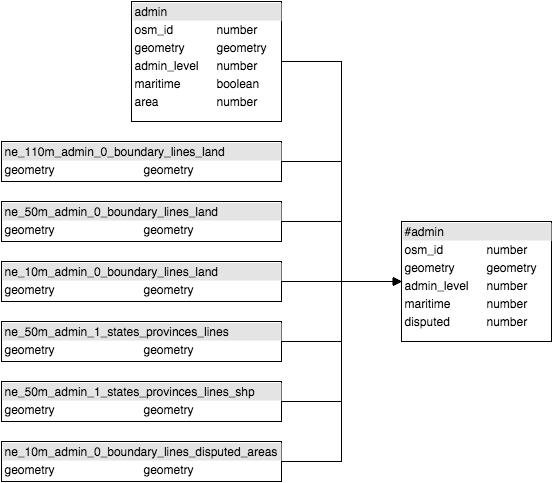
\includegraphics[scale=0.6]{images/admin_layer.png}
  \caption{Layers for administrative areas}
\end{figure}

\newpage
Roads are split up into normal roads, tunnels and bridges.

\begin{figure}[h]
  \centering
  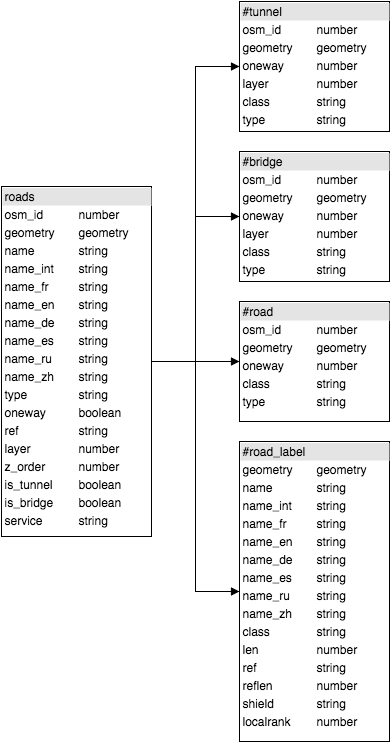
\includegraphics[scale=0.6]{images/road_layer.png}
  \caption{Layers for roads, tunnels and bridges}
\end{figure}

\newpage
Point of interests 

\begin{figure}[h]
  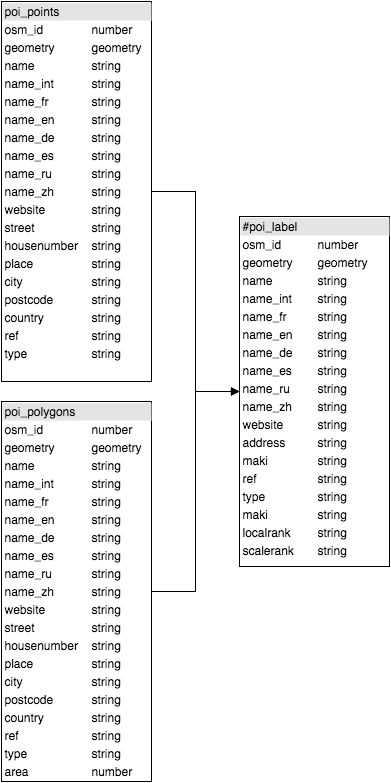
\includegraphics[scale=0.6]{images/poi_layer.png}
  \caption{Point of interest label layer}
\end{figure}


\newpage
Water bodies for lower zoom levels are taken from Natural Earth
data while lakes and rivers are from OpenStreetMap.

\begin{figure}[h]
  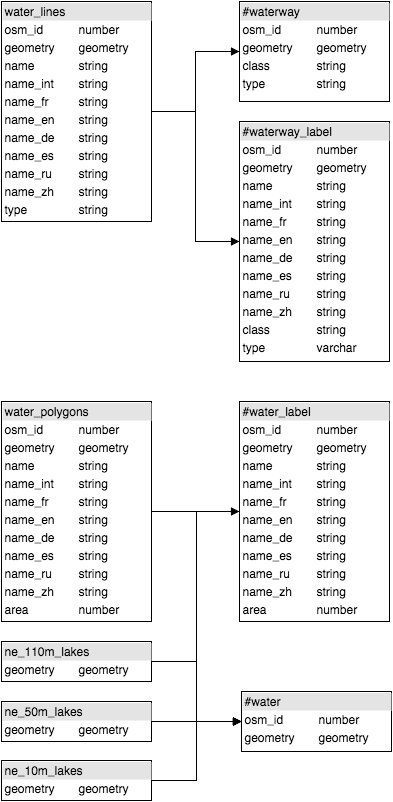
\includegraphics[scale=0.6]{images/water_layer.png}
  \caption{Water bodies and river layers}
\end{figure}



\newpage
The original OpenStreetMap place data is enriched with scalerank data
from natural earth.

\begin{figure}[h]
  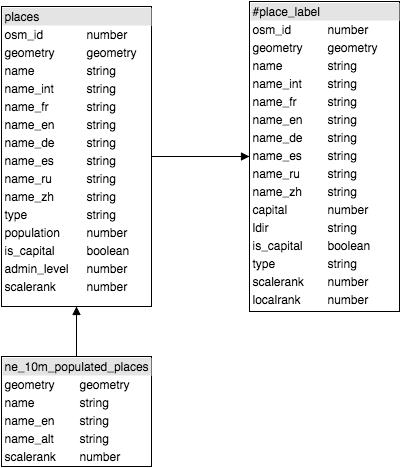
\includegraphics[scale=0.6]{images/place_layer.png}
  \caption{Place label layer}
\end{figure}




%------------------------------------------------------
\section{Package Diagrams}


%------------------------------------------------------
\section{Workflow}\label{workflow}

\paragraph{First step: Getting OSM
data}\label{first-step-getting-osm-data}

There are many different sources available to get OSM data from. Most of
the time Geofabrik\footnote{\url{http://download.geofabrik.de/}} was
referenced for getting single countries, continents or even the whole
planet. But many times people only need a single city or region, because
of this demand
Mapzen\footnote{\url{https://mapzen.com/data/metro-extracts/}} provides
OSM data for many cities and regions around the globe.

The OSM data is missing something very important: the administrative
boundaries. This needs to be downloaded separatly due to the fact, that
somebody could manipulate the boundary of a region. As a result of this
administrative boundaries get checked by the OSM community and released
separatly.

The data is available in the PBF and OSM XML format. If available the
PBF(Protocolbuffer Binary
Format)\footnote{\url{http://wiki.openstreetmap.org/wiki/PBF_Format}}
version should be choosen, as it is 30\% smaller and 5-6 times faster to
read and write than the bzipped OSM XML version.

\paragraph{Second step: Importing OSM data into
Postgis}\label{second-step-importing-osm-data-into-postgis}


\subsubsection{Third step: Mapbox studio source
project}\label{third-step-mapbox-studio-source-project}

A Mapbox studio source project is divided into the following folder
structure\footnote{\url{https://www.mapbox.com/guides/source-manual/\#source-project}}:

\begin{verbatim}
source-project.tm2source/
    data.yml
    data.xml
    .thumb.png
\end{verbatim}

The data file defines all feature sets(layers) like landuse, waterway,
road etc. The definition contains metadata like id, datasource(db, host,
query, srid, extent), description, fields and properties. Mapbox Studio
needs the yml version and mapnik the xml version of this file.
.thumb.png is a thumbnail image that gets displayed in the projects
list.

\subsubsection{Fourth step: Generating vector
tiles}\label{fourth-step-generating-vector-tiles}

To generate the vector tiles we use mapnik. Mapbox provides a very handy
tool to generate vector tiles.

\begin{verbatim}
tilelive-copy --bounds=-180,-85,180,85 bridge:///home/mapbox/tmp/project.tm2source/data.xml mbtiles:///tmp/project.mbtiles
\end{verbatim}

tilelive-copy provides the Mapnik XML file and the extent to mapnik
which then generates the vector tiles. Tilelive-copy outputs these
vector tiles in the mbtiles container.
